\documentclass[titlepage]{article}

\usepackage[margin=1in]{geometry}
\usepackage{csquotes}
\usepackage{fancyhdr}
\usepackage{marginnote}
\usepackage{enumitem}
\usepackage{xr}
\usepackage[style=chem-acs]{biblatex}
\usepackage{float,subcaption}
\usepackage{graphicx}
\usepackage{tikz}
\usepackage{siunitx}
\usepackage{amsmath,amssymb}
\usepackage{bm}
\usepackage{mhchem,chemfig}
\usepackage[hidelinks]{hyperref}

\MakeOuterQuote{"}

\fancypagestyle{main}{
    \fancyhf{}
    \fancyhead[L]{\leftmark}
    \fancyhead[R]{CHEM 22100}
    \fancyfoot[R]{Labalme\ \thepage}
}
\fancypagestyle{plain}{
    \fancyhead{}
    \renewcommand{\headrulewidth}{0pt}
}

\reversemarginpar

\setitemize[3]{label={\scriptsize$\blacksquare$}}

\DefineBibliographyStrings{english}{bibliography={References}}

\usetikzlibrary{decorations,arrows.meta,bending,calc}
\colorlet{rex}{magenta}
\colorlet{gax}{gray!50}
\colorlet{orx}{orange!90!yellow!95!black!90}

\sisetup{range-phrase=-,range-units=single}
\DeclareSIUnit{\calorie}{cal}
\DeclareSIUnit{\atomicmassunit}{amu}

\setchemfig{atom sep=2em,fixed length=true,bond offset=3pt,cram width=3pt}
\setcharge{extra sep=3pt}
\pgfdeclaredecoration{ddbond}{initial}{
    \state{initial}[width=3.5pt]{
        \pgfpathlineto{\pgfpoint{4pt}{0pt}}
        \pgfpathmoveto{\pgfpoint{0pt}{2pt}}
        \pgfpathlineto{\pgfpoint{1pt}{2pt}}
        \pgfpathmoveto{\pgfpoint{3pt}{2pt}}
        \pgfpathlineto{\pgfpoint{4pt}{2pt}}
        \pgfpathmoveto{\pgfpoint{4pt}{0pt}}
    }
    \state{final}{
        \pgfpathlineto{\pgfpointdecoratedpathlast}
    }
}
\tikzset{
    lddbond/.style={decorate,decoration=ddbond},
    rddbond/.style={decorate,decoration={ddbond,mirror}}
}

\newcommand{\e}[1][]{\text{e}^{#1}}

\usepackage{subfiles}

\addbibresource{../../main.bib}

\title{Spectral Analysis of Unknown G}
\author{
    Steven Labalme\\
    \normalsize Lab Section 1A05
}

\begin{document}




\maketitle



\pagestyle{main}
\renewcommand{\leftmark}{Written Assignment 2}
\setitemize{label={--}}
\noindent What is the letter/number of your unknown?



\section*{MS Data}
\begin{enumerate}
    \item What is the molecular weight of the molecular ion (M+), and therefore the molecular weight of your unknown?
    \item Does your unknown contain any \ce{Br} atoms? \ce{Cl}? Odd number of \ce{N}? Why or why not?
    \item Give a molecular formula for your product if it contains no oxygens. Give the molecular formulas if your product contains one or two oxygens (some may not be possible).
    \item Calculate the index of hydrogen deficiency, and therefore the number of rings and/or $\pi$-bonds in your unknown for each of the molecular formulas in Question 3. Show your calculations.
\end{enumerate}



\section*{IR Data}
\begin{enumerate}
    \item Is there a carbonyl in your unknown? State how you know. If one is present, state how the frequency narrows down the functional group it is a part of (carboxylic acid, ketone, aldehyde, ester, amide).
    \item What functional groups are present in your unknown molecule? For each, correlate the functional group with the frequency of the identifying peak.
    \item For each of the molecular formulas you listed in Question 3 of the MS Data section, state if these functional groups support or rule out the formula.
    \item List all the IR data from Questions 1 and 2 in ACS journal style. The format is: IR $\nu$max (ATR) \emph{list major peaks here} \si{\per\centi\meter}.
\end{enumerate}



\section*{\ce{{}^13C} NMR Data}
\begin{enumerate}
    \item Identify the solvent peak in the spectrum and list its chemical shift.
    \item Other than the solvent peak, how many signals are present in the \ce{{}^13C} NMR and how does this correlate to the number of chemically distinct carbons?
    \item Based on the chemical shifts, what functional groups are present in your compound? For each, correlate the functional group with the chemical shift of the identifying peak.
    \item For each of the molecular formulas you listed in Question 3 in the MS Data section, state if your \ce{{}^13C} NMR data supports or rules out the formula.
    \item What molecular formula(s) are supported by both the IR and \ce{{}^13C} NMR data?
    \item List all the \ce{{}^13C} NMR data in ACS journal style. The format is: \ce{{}^13C} NMR (\SI{125}{\mega\hertz}, \ce{CDCl3}): $\delta$ \emph{list chemical shifts here}.
\end{enumerate}



\section*{\ce{{}^1H} NMR Data}
\begin{enumerate}
    \item List the integration of all peaks as a ratio. For example, 4-hydroxy-4-methyl-2-pentanone would have a ratio of $1:2:3:6$. How does the integration of the peaks correlate to the number of hydrogens present in the molecule?
    \item For the molecular formula(s) listed in Question 5 of the \ce{{}^13C} NMR Data section, state if the integration data supports or rules out the formula(s).
    \item Based on the chemical shifts, what functional groups are present in your compound? For each, correlate the functional group with the chemical shift of the identifying peak.
    \item State how the functional groups identified in the \ce{{}^1H} NMR data correlate with the functional groups identified in the \ce{{}^13C} NMR and IR data. If there are any molecular formula(s) ruled out by this data, state that as well.
    \item For each peak in the \ce{{}^1H} NMR spectrum, state the splitting pattern and how many neighboring hydrogens this correlates to. Example: singlet - 0 neighboring hydrogens.
    \item For each peak, draw a partial structure that uses all three pieces of information (chemical shift, integration, splitting patterns). Make sure that you highlight the hydrogen atom or atoms that are responsible for the signal. An example of this is \ce{-R-CO-C\textbf{H}2-R} or
    \begin{center}
        \footnotesize
        \chemfig{R-[:30](=[2]O)-[:-30](-[:-70]\textbf{H})(-[:-110]\textbf{H})-[:30]R}
    \end{center}
    \item List all the \ce{{}^1H} NMR data in ACS journal style. The format is: \ce{{}^1H} NMR (\SI{500}{\mega\hertz}, \ce{CDCl3}): $\delta$ \emph{chemical shift} (\emph{splitting}, \emph{integration}). As an example, the following peak would be reported as: \ce{{}^1H} NMR (\SI{80}{\mega\hertz}, \ce{CDCl3}): $\delta$ 1.75 (sextet, 2H)
    \begin{center}
        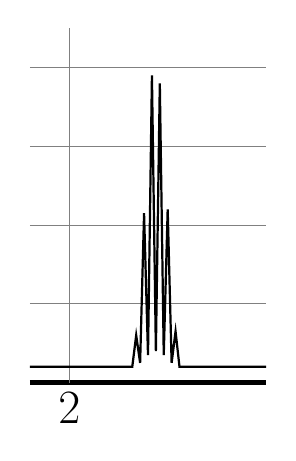
\begin{tikzpicture}
            \draw [ultra thick] (0,0) -- (3,0);
            \draw [gray]
                (0.5,0) node[below,black]{\LARGE 2} -- ++(0,4.5)
                (0,4) -- ++(3,0)
                (0,3) -- ++(3,0)
                (0,2) -- ++(3,0)
                (0,1) -- ++(3,0)
            ;
    
            \draw [thick] (0,0.2)
                -- (1.30,0.20)
                -- (1.35,0.60)
                -- (1.40,0.25)
                -- (1.45,2.15)
                -- (1.50,0.35)
                -- (1.55,3.90)
                -- (1.60,0.40)
                -- (1.65,3.80)
                -- (1.70,0.35)
                -- (1.75,2.20)
                -- (1.80,0.25)
                -- (1.85,0.65)
                -- (1.90,0.20)
                -- (3.00,0.20)
            ;
        \end{tikzpicture}
    \end{center}
\end{enumerate}



\section*{Final Structure}
\begin{enumerate}
    \item Piece together a complete structure of your unknown using everything that you have listed so far into a drawing using chemical drawing software.
    \item Locate published IR and \ce{{}^1H} NMR spectra for your proposed structure and compare them to the spectra you received. Discuss why these published spectra prove the identity of your unknown or disprove your proposed structure. Be sure to correlate all data referenced in the IR and \ce{{}^1H} NMR sections. Include the spectra and citations in your report.
\end{enumerate}




\end{document}